\section{Results}
\begin{frame}{}
    \LARGE GANs: \textbf{Results}
\end{frame}

\begin{frame}[allowframebreaks]{Results}
\begin{figure}
    \centering
    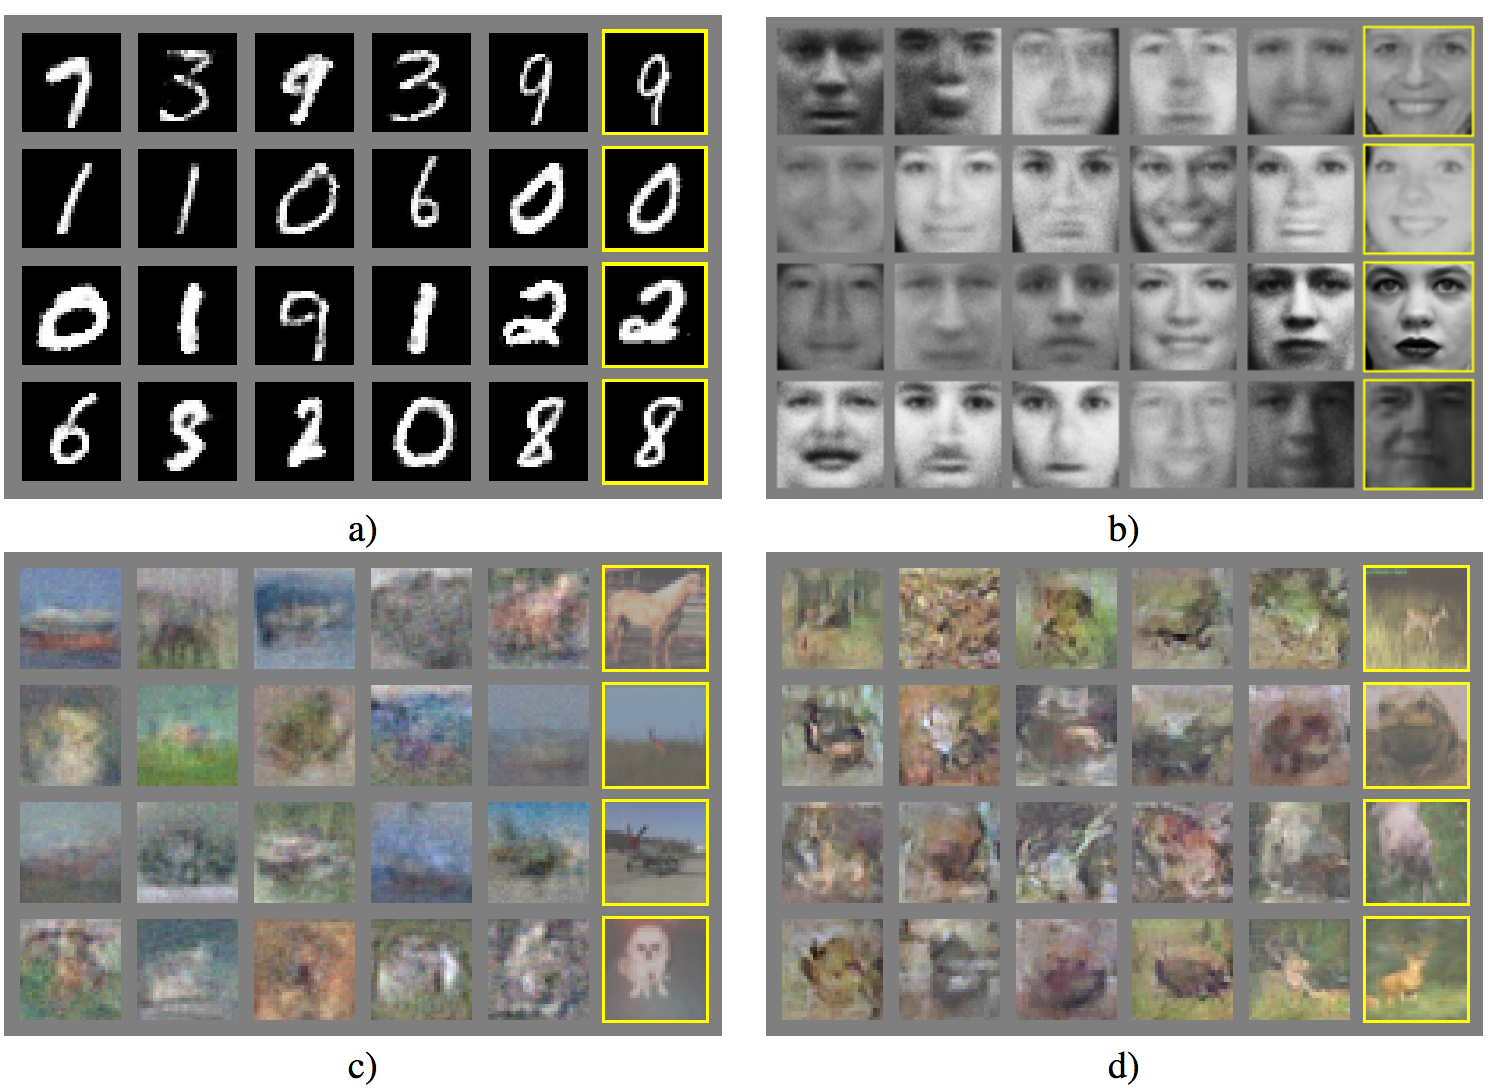
\includegraphics[height=0.8\textheight, width=\textwidth, keepaspectratio]{images/gan/result-goodfellow.png}
    \caption*{Figure from Goodfellow et al 2014, showing GAN results on various datasets.}
\end{figure}

\framebreak
\begin{figure}
    \centering
    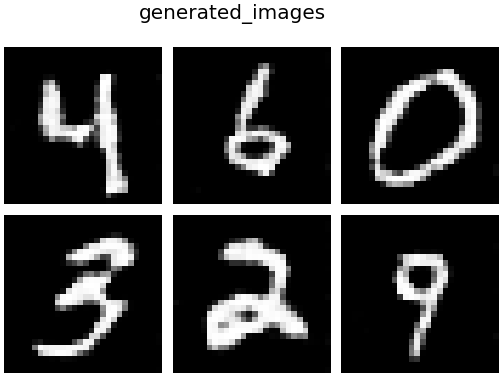
\includegraphics[height=0.8\textheight, width=\textwidth, keepaspectratio]{images/gan/gan_results_mnist.png}
    \caption*{GAN generated samples for MNIST digits dataset}
\end{figure}

\framebreak
\begin{figure}
    \centering
    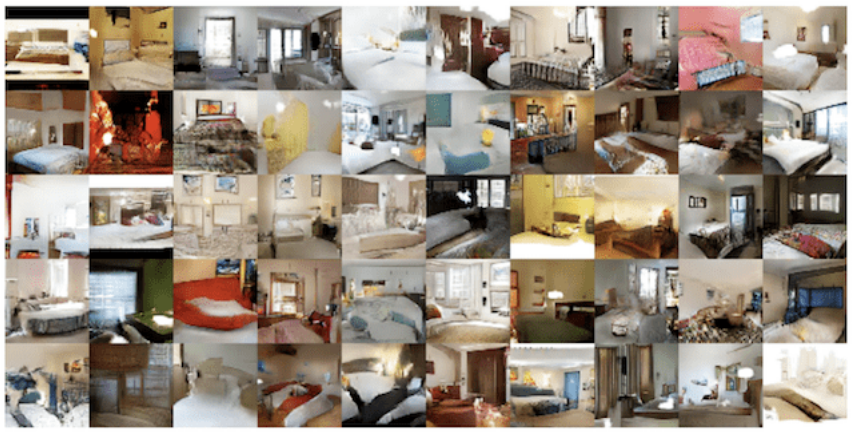
\includegraphics[height=0.8\textheight, width=\textwidth, keepaspectratio]{images/gan/gan_results_2.png}
    \caption*{GAN generated samples for bedroom images. {\scriptsize [Radford, Metz \& Chintala, ICLR 2016, Fig.~3]}}
\end{figure}

\framebreak
\begin{figure}
    \centering
    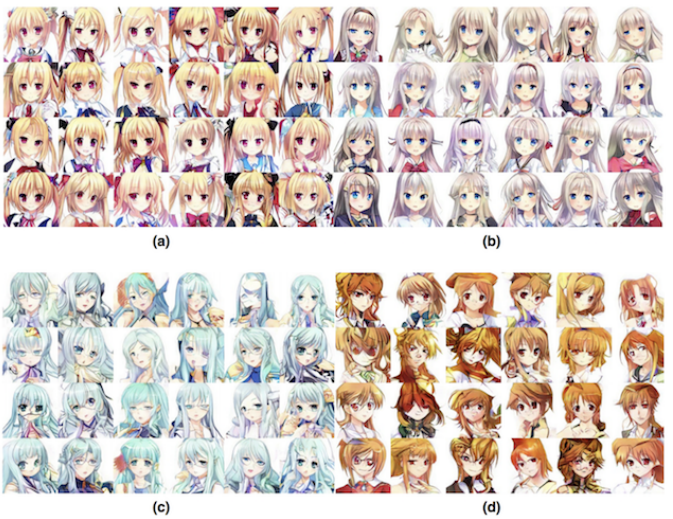
\includegraphics[height=0.72\textheight, width=\textwidth, keepaspectratio]{images/gan/gan_results_3.png}
    \caption*{GAN generated samples for anime character faces. {\scriptsize [Jin et al., ``Towards the Automatic Anime Characters Creation with GANs,'' 2017, Fig.~9]}}
\end{figure}
    
\end{frame}